% !TEX root = 0_tcc.tex
\clearpage

\section{Metodologia}

Foi considerado o sistema em regime quasi-estacionário, onde entre cada intervalo
de tempo é suposto que não há alteração na configuração do \acrshort{hres}.

A primeira etapa foi a avaliação e tratamento dos dados, de forma a encontrar
uma entrada que não tendencie a rede. Foi avaliado a quantidade de
\acrshort{nan}s, problema de falta de dados que pode comprometer a previsão.

A carga a ser abastecida pelo sistema é suposta periódica ao longo de cada dia,
com perfil de carga exibido na Figura~\ref{fig:perfil}. O perfil foi interpolado
para garantir maior granularidade na análise da carga. Foi obtida a
carga líquida renovável para cada instante da série temporal de acordo com a
Equação~\ref{eq:netload}.

\begin{equation}
  \label{eq:netload}   E_{\text{ren}} = E_L - E_w - E_s
\end{equation}

% !TEX root = ../0_tcc.tex

\begin{figure}[H]
	\centering
	\begin{subfigure}[b]{\textwidth}
		\centering
		\includegraphics[width=0.7\textwidth]{../img/load.png}
		\caption{Curva original}\label{fig:load}
	\end{subfigure}
	\\ \vspace{0.1cm}
	\begin{subfigure}[b]{\textwidth}
		\centering
		\includegraphics[width=0.7\textwidth]{../img/load_corr.png}
		\caption{Curva interpolada}\label{fig:load_corr}
	\end{subfigure}
	\caption{Perfil de carga de exemplo. Fonte: própria.}\label{fig:perfil}
\end{figure}


Os modelos a seguir foram considerados para cálculo de potência cada componente
do sistema.

\subsection{Solar}

A modelagem de um sistema fotovoltaico começa com o cálculo da irradiância
incidente no plano dos painéis. A irradiância $I_{T}$ é a soma da direta
$I_{b}$, difusa $I_{d}$ e a refletida $I_{r}$, proporcionais ao ângulo de
inclinação, de acordo com a Equação~\ref{eq:solar:it}.

\begin{equation}
  \label{eq:solar:it}   I_T = I_b R_b + I_d R_d + (I_b + I_d) R_r
\end{equation}

A potência dos painéis depende da área ocupada $A_{PV}$ e a eficiência $\eta$
dos módulos, de acordo com a Equação~\ref{eq:solar:p}.

\begin{align}
  \label{eq:solar:p}    P_{PV} &= I_T \eta A_{PV} \\
  \label{eq:solar:etam}    \eta_m &= \eta_r [1 - \beta (T_c - T_r)] \\
  \label{eq:solar:tc}   T_c &= T_a + \left(\frac{T_{\text{NOCT}}-20}{800}\right) I_T
\end{align}

O painel considerado foi o \emph{YGE 60 Cell Series 2}, com características na
Tabela~\ref{tbl:painel}.

% !TEX root = ../00_tcc.tex

\begin{table}[ht]
	\centering
	\caption{Painel YGE 60 Cell Series 2}\label{tbl:painel}
    \begin{tabular}{c r l}
		\hline
        Parâmetro    &   Valor & Unidade\\
		\hline
		\hline
        $\eta$       &  $19.6$ & $\cdot$  \\
        $\beta$      & $-0.30$ & T$^{-1}$ \\
        $A_{PV}$     &  $1.63$ & m$^2$    \\
		\hline
	\end{tabular}
\end{table}


\subsection{Eólica}

Para velocidade do vento medidas em uma altura diferente do cubo do aerogerador,
é preciso corrigir de acordo com a lei de cisalhamento vertical. As medições
mais próximas à superfície são menores devido ao à interação com o solo. A
medida que ascende-se, a velocidade torna-se logarítmicamente maior de acordo
com a Equação~\ref{eq:wind:pl}.

\begin{equation}
  \label{eq:wind:pl}  V_z = V_i \frac{Z}{Z_i}^x
\end{equation}

A curva de potência de um aerogerador é deduzida a partir de dados de campanhas
de medição do recurso eólico local.  Quando os dados disponíveis para o sistema
híbrido tem frequência diferente do que foi usado na campanha de medição, a
curva de potência original não é mais aplicável. Pode ser feita a correção da
curva introduzindo componentes estocásticas e determinísticas de acordo com o
modelo de Von-Kármán para rajadas de vento contínuas. Por motivos de
simplificação, foi considerado que a curva foi deduzida na mesma frequência
amostral da aplicação do sistema, dispensando correção.

A Turbina considerada foi o \emph{Bergey Excel-10}, com curva de potência na
Figura~\ref{fig:wind:power}. A curva também foi interpolada.

% !TEX root = ../00_tcc.tex

\begin{figure}[H]
	\centering
	\begin{subfigure}[b]{\textwidth}
		\centering
		\includegraphics[width=0.8\textwidth]{../img/bergey.png}
		\caption{Curva original}\label{fig:bergey}
	\end{subfigure}
	\\ \vspace{0.5cm}
	\begin{subfigure}[b]{\textwidth}
		\centering
		\includegraphics[width=0.8\textwidth]{../img/bergey_corr.png}
		\caption{Curva interpolada}\label{fig:bergey_corr}
	\end{subfigure}
	\caption{Curva de potência do aerogerador \emph{Bergey Excel-10}. Fonte: própria.}\label{fig:wind:power}
\end{figure}


\subsection{Diesel}

O grupo diesel ser modelado como uma função linear é uma suposição razoável de
acordo com resultados experimentais, como visto
em~\cite[cap.~6.1]{manwell2006hybrid2}. O coeficiente linear da função é o
consumo sem carga, com a máquina parada. A inclinação da reta é dada pela taxa
de consumo de combustível por unidade de potência de saída.  De acordo
com~\cite{Nema_2009}, para determinar a capacidade nominal do gerador diesel a
ser instalado, caso estiver diretamente conectado à carga, então o capacidade
nominal do gerador deve ser pelo menos igual à carga máxima.

\begin{align}
  \label{eq:diesel} F &= a + b P \\
  \nonumber a &= \text{consumo sem carga}\\
  \nonumber b &= \text{consumo por potência ($\ell$/kWh)}
\end{align}

O gerador diesel considerado foi o exemplo apresentado
em~\citeauthor{manwell2006hybrid2}, com características na
Tabela~\ref{tbl:diesel}.

% !TEX root = ../0_tcc.tex

\begin{table}[ht]
	\centering
	\caption{Gerador diesel}\label{tbl:diesel}
    \begin{tabular}{c r l}
		\hline
        Parâmetro        &  Valor & Unidade\\
		\hline
		\hline
        $P_{\text{nom}}$ &  $15$   & kW       \\
        $a$              &  $0$   & $\ell$/h   \\
        $b$              &  $1/3$   & {kWh}$^{-1}$    \\
		\hline
	\end{tabular}
\end{table}


\subsection{Bateria}

A capacidade do banco de baterias é dimensionado em função do tempo de
inatividade das outras fontes, referido como dias de autonomia.  Normalmente é
assumido 2 ou 3 dias de autonomia, ou seja: as baterias tem capacidade para
sustentar sozinhas o consumo por esse período.

As baterias são limitadas em um estado máximo e um mínimo de carga, não podendo
ultrapassá-los, como na Equação~\ref{eq:bat:lim}. O estado de carga pode ser
atualizado pelas equações~\ref{eq:bat:y1} e~\ref{eq:bat:y2} respeitando o modelo cinético de
baterias, \acrlong{kibam}.

\begin{equation}
  \label{eq:bat:lim}           \text{SOC}_{\text{min}} \leq \text{SOC}(t)   \leq \text{SOC}_{\text{max}}
\end{equation}

O \acrshort{kibam} consiste em admitir que um parte da capacidade está a
disposição para ser consumida imediadamente (\emph{available charge}) e outra
está confinada (\emph{bound charge}). Tal fato decorre da inércia da bateria em
transformar energia química em energia elétrica prontamente disponível para o
consumo.  O modelo restringe a mudança de carga de acordo com a
equação~\ref{eq:bat:y1} para a carga confinada e a equação~\ref{eq:bat:y2} para
carga disponível. Cada bateria possui um parâmetro $c$ que representa o
percentual de carga disponível e outo $k$ que mensura a velocidade de conversão
de energia.

\begin{align}
  \label{eq:bat:y1}    q_a(t+1) &= q_a r + \frac{(q_a k' c - i) (1 - r) - i c (k' t - 1 + r)}{k'} \\
  \label{eq:bat:y2}    q_b(t+1) &= q_b r + q_t (1 - c) (1 - r) - \frac{i (1 - c) k' t - 1 + r}{k'}
\end{align}

A bateria usada foi a \emph{Trojan Solar SPRE 12 225}, com especificações na
Tabela~\ref{tbl:bateria}.

% !TEX root = ../0_tcc.tex

\begin{table}[ht]
	\centering
	\caption{Bateria Trojan SPRE 12 225}\label{tbl:bateria}
    \begin{tabular}{c r l}
		\hline
		Parâmetro    &   Valor & Unidade\\
		\hline
		\hline
		$V$                         &  $12$    & V       \\
		$E_{\text{max}}$            &  $225$   & Ah      \\
		$\eta$                      &  $75\%$  & $\cdot$ \\
		$\text{SOC}_{\text{min}}$   &  $40\%$  & $\cdot$ \\
		$\text{SOC}_{\text{max}}$   &  $100\%$ & $\cdot$ \\
		\hline
	\end{tabular}
\end{table}


\subsection{Rede Neural}

A metodologia para previsão foi usar 36 instantes passados de tempo para prever
o comportamento meteorológico dos próximos 36 instantes.  Para isso, 36 redes
neurais foram treinadas, cada uma com o objetivo de prever um instante futuro
específico. A rede 1 prevê o instante $t+1$, a rede 2 prevê o instante $t+2$ e
assim em diante até a trigésima sexta. Todas recebem a mesma entrada, os 36
instantes passados, como ilustrado na Figura~\ref{tikz:nns}.  As séries
temporais usadas foram a de radiação solar e a velocidade do vento, cada uma com
suas respectivas previsões, totalizando 72 \acrshort{ann}s.

% !TEX root = ../0_tcc.tex

\begin{figure}[ht]
	\centering
		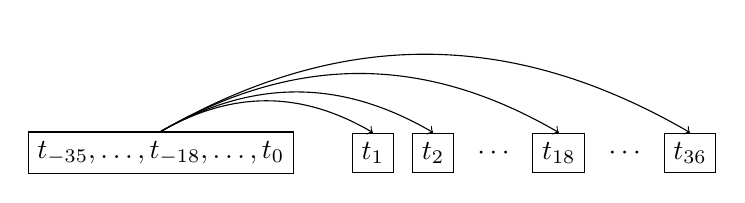
\begin{tikzpicture}
			\node[draw, rectangle]  at  (0,0)  (ts-36)
			{$t_{-35}, \dots, t_{-18}, \dots, t_{0} $};

			\node[draw, rectangle] at ([xshift=1cm]ts-36.east)   (ts1)   {$t_1$};
			\draw[->]  (ts-36.north) [bend left] to (ts1.north)  ;

			\node[draw, rectangle] at ([xshift=0.5cm]ts1.east)   (ts2)   {$t_2$};
			\draw[->]  (ts-36.north) [bend left] to (ts2.north)  ;

			\node[] at ([xshift=0.5cm]ts2.east)   (tsdot) {$\cdots$};

			\node[draw, rectangle] at ([xshift=0.5cm]tsdot.east) (ts18)  {$t_{18}$};
			\draw[->]  (ts-36.north) [bend left] to (ts18.north)  ;

			\node[] at ([xshift=0.5cm]ts18.east)   (tsdot2) {$\cdots$};

			\node[draw, rectangle] at ([xshift=0.5cm]tsdot2.east)  (ts36)  {$t_{36}$};
			\draw[->]  (ts-36.north) [bend left] to (ts36.north)  ;
		\end{tikzpicture}
	\caption{Esquema de várias redes para previsão individual de timesteps. Fonte: própria.}\label{tikz:nns}
\end{figure}


A arquitetura para todas redes foi a mesma, composta células \acrshort{rnn}
simples. O modelo foi feito utilizando o \emph{Keras}. A ferramenta é uma
\acrshort{api} do \emph{TensorFlow}, biblioteca de aprendizado de máquina
desenvolvida pelo \emph{Google}.  Para treinamento e teste da rede foi usado a
plataforma \emph{Google Colab} que permite computação em nuvem com
disponibilidade de \acrshort{gpu}. Outras arquiteturas foram avaliadas como a
\acrshort{lstm} mas, como obteve resultados semelhantes à \acrshort{rnn}, foi
escolhida a mais simples.

Os dados que entram na rede foram normalizados: subtraídos do menor valor e
divididos de pela diferença entre máximo e mínimo. O processo ilustrado pela
Equação~\ref{eq:minmax} tem objetivo de limitar os dados no intervalo de [0, 1].
Dessa forma, evita-se problemas de cálculo numérico como \emph{overflow} durante
o processo de treinamento e o gradiente descendente é capaz de convergir muito
mais rápido.

\begin{equation}
  \label{eq:minmax}   x_{i}' = \frac{x_{i} - x_{\text{min}}}{x_{\text{max}} - x_{\text{min}}}
\end{equation}

Além das células \acrshort{rnn}, também foi usado \emph{dropout}. A técnica
consiste em aleatoriamente desativar um percentual determinado de neurônios de
uma camada. Os neurônios desativados não passam informação à próxima camada.
Dessa forma, no processo de treinamento, a rede aprende a não depender de cada
neurônio individualmente, reduzindo a probabilidade de um nodo enviesar toda a
\acrshort{ann}. O sumário da rede é exibido na Tabela~\ref{tbl:model}.

% !TEX root = ../0_tcc.tex

\begin{table}[ht]
	\centering
	\caption{Modelo treinado}\label{tbl:model}
	\begin{subtable}{\textwidth}
		\centering
		\caption{Arquitetura}\label{tbl:model_arq}
		\begin{tabular}{c c c}
			\hline
			Camada   &   Shape de saída    &   Parâmetros\\
			\hline
			\hline
			SimpleRNN&   (None, 36, 64)   &   4224      \\
			Dropout  &   (None, 36, 64)   &   0         \\
			SimpleRNN&   (None, 32)       &   3104      \\
			Dropout  &   (None, 32)       &   0         \\
			Dense    &   (None, 1)        &   33        \\
			\hline
		\end{tabular}
	\end{subtable}
	\\ \vspace{1cm}
	\begin{subtable}{\textwidth}
		\centering
		\caption{Parâmetros}\label{tbl:model_param}
		\begin{tabular}{c c c}
			\hline
			Total de parâmetros & Parâmetros treináveis & Parâmetros não treináveis \\
			\hline
			\hline
			7,361        &    7,361         & 0 \\
			\hline
		\end{tabular}
	\end{subtable}
\end{table}


\subsection{Sistema Híbrido}

Foi considerado um sistema abastecido por 10 módulos fotovoltaicos, 1
aerogerador, 1 gerador diesel e banco de bateria com 1 dia de autonomia, como
mostrado na Tabela~\ref{tbl:sistema}.
Dessa forma, a tensão do barramento de corrente contínua ficou em 300 volts de
fotovoltaica mais 220 volts do aerogerador, totalizando 520.

% !TEX root = ../00_tcc.tex

\begin{table}[ht]
	\centering
	\caption{Sistema híbrido abordado}\label{tbl:sistema}
    \begin{tabular}{l l l}
		\hline
        Equipamento  &  Modelo     & Quantidade    \\
		\hline
		\hline
        Aerogerador          & Bergey Excel-10          & 1               \\
        Painel               & YGE 60 CELL Series 2     & 10              \\
		Gerador Diesel 15 kW &                          & 1               \\
		Baterias             & Trojan Solar SPRE 12 225 & 20              \\
		\hline
	\end{tabular}
\end{table}


Foi feita uma comparação considerando a \acrshort{lpsp} para as duas
estratégias: \acrshort{lf}.  O gerador diesel em
\acrshort{lf} entrará em operação caso a bateria não suprir o déficit,
acompanhando a carga líquida.  Em \acrshort{cc}, quando há déficit de energia, o
gerador diesel é ligado na máxima potência disponível que não gere excesso,
escoando a sobra para a bateria. Para manter a vida útil do gerador, tempos
mínimos de operação foram considerados.
